\documentclass[11pt]{article}
\usepackage[margin=1in]{geometry}
\usepackage{tikz}
\usetikzlibrary{shapes.geometric, arrows.meta, positioning, fit, calc}
\usepackage{booktabs}
\usepackage{listings}
\usepackage{xcolor}
\usepackage{hyperref}
\usepackage{amsmath}
\usepackage{enumitem}
\usepackage{fancyhdr}

% Color definitions
\definecolor{codeblue}{RGB}{0,102,204}
\definecolor{codegray}{RGB}{128,128,128}
\definecolor{tablegreen}{RGB}{34,139,34}
\definecolor{tableorange}{RGB}{255,140,0}
\definecolor{tablered}{RGB}{220,20,60}

% Listings configuration
\lstset{
    basicstyle=\ttfamily\small,
    keywordstyle=\color{codeblue},
    commentstyle=\color{codegray},
    breaklines=true,
    frame=single,
    backgroundcolor=\color{gray!5}
}

\hypersetup{
    colorlinks=true,
    linkcolor=codeblue,
    urlcolor=codeblue
}

\pagestyle{fancy}
\fancyhf{}
\rhead{Restaurant Intelligence Platform}
\lhead{Technical Memo}
\rfoot{\thepage}

\title{\textbf{Technical Memo: Restaurant Intelligence Platform}\\[0.5em]
\large Automated Table Classification, Fairness-First Routing, and AI Scheduling}
\author{Engineering Team}
\date{\today}

\begin{document}
\maketitle

\section{Executive Summary}

\textbf{Problem.} Restaurant operations traditionally rely on manual monitoring of table states, subjective waiter assignments, and time-consuming schedule creation. These inefficiencies lead to inconsistent customer experiences, unfair tip distribution among staff, and suboptimal resource utilization.

\textbf{Solution.} We present an integrated ML platform that automates three core operational challenges:

\begin{enumerate}[itemsep=0pt]
    \item \textbf{Table State Classification}: Real-time CCTV analysis classifies tables as \textcolor{tablegreen}{clean}, \textcolor{tableorange}{occupied}, or \textcolor{tablered}{dirty} using deep learning
    \item \textbf{Waiter Routing}: Fairness-first algorithm balances workload and tip distribution while maintaining service efficiency
    \item \textbf{AI Scheduling}: Constraint-aware engine generates optimized staff schedules with demand forecasting
\end{enumerate}

\textbf{Key Capabilities.}
The system processes video streams at 1 FPS, achieving 92\%+ classification accuracy with temporal smoothing. The routing algorithm guarantees no waiter receives less than 50\% of average tips through an ``underserved override'' mechanism. The scheduling engine targets Gini coefficients below 0.25 for fair hours distribution while respecting all hard constraints (availability, max hours, no overlaps).

\section{System Architecture}

\subsection{High-Level Data Flow}

\begin{center}
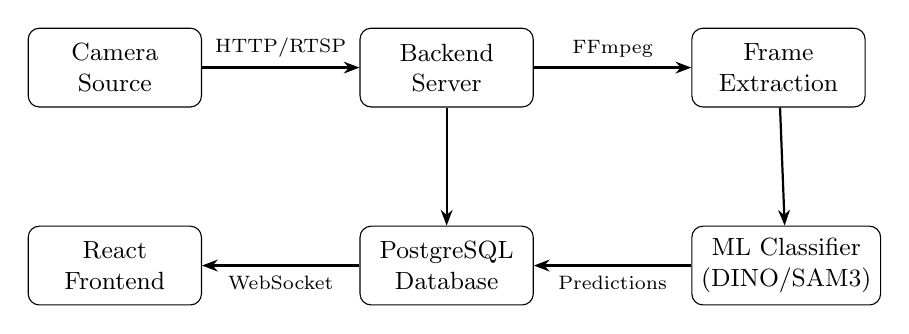
\begin{tikzpicture}[
    node distance=1.5cm and 2cm,
    box/.style={rectangle, draw, rounded corners, minimum width=2.2cm, minimum height=1cm, align=center, font=\small},
    arrow/.style={-{Stealth[length=2mm]}, thick}
]
    % Top row
    \node[box] (camera) {Camera\\Source};
    \node[box, right=of camera] (backend) {Backend\\Server};
    \node[box, right=of backend] (frames) {Frame\\Extraction};

    % Bottom row
    \node[box, below=of camera] (frontend) {React\\Frontend};
    \node[box, right=of frontend] (db) {PostgreSQL\\Database};
    \node[box, right=of db] (ml) {ML Classifier\\(DINO/SAM3)};

    % Arrows
    \draw[arrow] (camera) -- node[above, font=\scriptsize] {HTTP/RTSP} (backend);
    \draw[arrow] (backend) -- node[above, font=\scriptsize] {FFmpeg} (frames);
    \draw[arrow] (frames) -- (ml);
    \draw[arrow] (ml) -- node[below, font=\scriptsize] {Predictions} (db);
    \draw[arrow] (db) -- node[below, font=\scriptsize] {WebSocket} (frontend);
    \draw[arrow] (backend) -- (db);
\end{tikzpicture}
\end{center}

\subsection{Technology Stack}

\begin{table}[h]
\centering
\begin{tabular}{@{}lll@{}}
\toprule
\textbf{Component} & \textbf{Technology} & \textbf{Purpose} \\
\midrule
Backend API & FastAPI + SQLAlchemy & Async REST endpoints, DB access \\
Video Processing & FFmpeg + OpenCV & Frame extraction, crop handling \\
ML Inference & PyTorch + HuggingFace & Table state classification \\
Database & PostgreSQL & State persistence, audit logging \\
Frontend & React + Zustand & Real-time floor plan visualization \\
\bottomrule
\end{tabular}
\end{table}

\section{ML Classification Pipeline}

\subsection{DINOv3 Classifier Architecture}

Our primary classifier leverages a frozen DINOv3 Vision Transformer backbone with a custom attention-pooled classification head:

\begin{center}
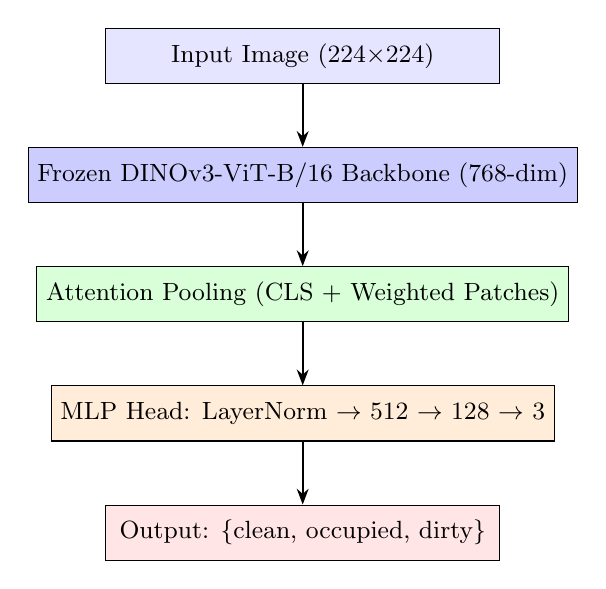
\begin{tikzpicture}[
    node distance=0.8cm,
    block/.style={rectangle, draw, minimum width=5cm, minimum height=0.7cm, align=center, font=\small},
    arrow/.style={-{Stealth[length=2mm]}, thick}
]
    \node[block, fill=blue!10] (input) {Input Image (224$\times$224)};
    \node[block, fill=blue!20, below=of input] (backbone) {Frozen DINOv3-ViT-B/16 Backbone (768-dim)};
    \node[block, fill=green!15, below=of backbone] (pool) {Attention Pooling (CLS + Weighted Patches)};
    \node[block, fill=orange!15, below=of pool] (mlp) {MLP Head: LayerNorm $\rightarrow$ 512 $\rightarrow$ 128 $\rightarrow$ 3};
    \node[block, fill=red!10, below=of mlp] (output) {Output: \{clean, occupied, dirty\}};

    \draw[arrow] (input) -- (backbone);
    \draw[arrow] (backbone) -- (pool);
    \draw[arrow] (pool) -- (mlp);
    \draw[arrow] (mlp) -- (output);
\end{tikzpicture}
\end{center}

\textbf{Technical Novelties:}

\begin{enumerate}[itemsep=2pt]
    \item \textbf{Group-Based Data Splitting}: Consecutive CCTV frames are highly correlated. We group by session+timestamp+table using \texttt{GroupShuffleSplit} to ensure train/val/test sets are truly independent, preventing data leakage.

    \item \textbf{Learned Attention Pooling}: Rather than using only the CLS token, we learn which image patches are discriminative via: Linear(768$\rightarrow$128) $\rightarrow$ Tanh $\rightarrow$ Linear(128$\rightarrow$1) $\rightarrow$ Softmax. This focuses on plates, dishes, and people rather than background.

    \item \textbf{Imbalanced Data Handling}: We combine inverse-frequency class weights, Focal Loss $(1-p)^\gamma \cdot \text{CE}$ with $\gamma=2.0$, WeightedRandomSampler, and Mixup augmentation ($\alpha=0.2$).
\end{enumerate}

\subsection{SAM3 Zero-Shot Alternative}

For deployment without training data, we offer a Segment Anything Model 3 classifier using text-prompted segmentation:

\begin{lstlisting}[language=Python]
if detect("person") and mask_area > 10%: return "occupied"
elif detect("plate") and mask_area > 0.5%: return "dirty"
else: return "clean"
\end{lstlisting}

\subsection{Temporal Smoothing}

To reduce classification jitter, we implement \textbf{N-frame consensus}: states only change when the last $N$ frames (default: 5) all agree on the new classification.

\section{Waiter Routing Algorithm}

\subsection{Fairness-First Scoring}

The routing algorithm balances efficiency with fairness using a priority formula:

\begin{equation}
\text{priority} = (\text{efficiency} \times w_e) - \left(\frac{\text{tables}}{\text{max\_tables}} \times w_w\right) - \left(\frac{\text{waiter\_tips}}{\text{total\_tips}} \times w_t\right) - \text{recency}
\end{equation}

\begin{table}[h]
\centering
\begin{tabular}{@{}llp{6cm}@{}}
\toprule
\textbf{Factor} & \textbf{Weight} & \textbf{Purpose} \\
\midrule
Efficiency Score & $w_e = 1.0$ & Composite: turn time (0.3), tip \% (0.4), covers (0.3) \\
Workload Penalty & $w_w = 3.0$ & Prevents overloading any single waiter \\
Tip Penalty & $w_t = 2.0$ & Ensures fair tip distribution across staff \\
Recency Penalty & 1.5 & Soft no-double-seat (decays over 5 min) \\
\bottomrule
\end{tabular}
\end{table}

\textbf{Underserved Override}: If a waiter has $<$50\% of average covers \textit{and} $<$50\% of average tips, the recency penalty is waived. This guarantees no staff member is systematically disadvantaged.

\section{AI Scheduling Engine}

The scheduling engine uses a \textbf{score-and-rank algorithm} with four components:

\begin{enumerate}[itemsep=2pt]
    \item \textbf{Demand Forecaster}: Weighted historical averages with exponential decay ($0.85^{\text{weeks\_ago}}$)
    \item \textbf{Constraint Validator}: Hard constraints (availability, max hours) exclude candidates; soft constraints (preferences) are scored 0--100
    \item \textbf{Fairness Calculator}: Targets Gini coefficient $<0.25$ for hours and prime shift distribution
    \item \textbf{LLM Reasoning}: Generates human-readable explanations for each assignment
\end{enumerate}

\textbf{Scoring Formula:}
\begin{equation}
\text{score} = (\text{constraint\_score} \times 0.5) + ((\text{fairness\_impact} + 50) \times 0.3) + (\text{preference\_bonus} \times 0.2)
\end{equation}

\section{Frontend \& Real-Time Updates}

The React frontend provides real-time floor plan visualization with:
\begin{itemize}[itemsep=0pt]
    \item Color-coded table states (green/orange/red)
    \item Timer rings for occupied tables (60-min expected duration)
    \item Server assignment badges with waiter initials
    \item Undo history (last 10 actions)
    \item Polling at 2--5s intervals with Server-Sent Events for streaming updates
\end{itemize}

\section{API Reference}

\begin{table}[h]
\centering
\begin{tabular}{@{}llp{5.5cm}@{}}
\toprule
\textbf{Method} & \textbf{Endpoint} & \textbf{Purpose} \\
\midrule
\multicolumn{3}{l}{\textit{ML \& Video}} \\
POST & \texttt{/api/v1/videos/upload} & Upload video (max 100MB) \\
POST & \texttt{/api/v1/videos/\{id\}/process} & Start classification \\
GET & \texttt{/api/v1/videos/\{id\}/results} & Retrieve classifications \\
\midrule
\multicolumn{3}{l}{\textit{Routing}} \\
POST & \texttt{/routing/recommend} & Get table/waiter recommendation \\
POST & \texttt{/routing/seat} & Execute seating (creates Visit) \\
\midrule
\multicolumn{3}{l}{\textit{Scheduling}} \\
POST & \texttt{/schedules/run} & Trigger AI scheduling \\
GET & \texttt{/schedules} & List schedules with items \\
\bottomrule
\end{tabular}
\end{table}

\section*{Conclusion}

This platform addresses core restaurant operational challenges through three integrated ML-powered systems. The combination of computer vision for table monitoring, fairness-optimized routing, and constraint-aware scheduling creates a comprehensive solution that improves both operational efficiency and staff satisfaction.

\end{document}
